%In this section, the layer is described in some detail in terms of its specific subsystems. Describe each of the layers and its subsystems in a separate chapter/major subsection of this document. The content of each subsystem description should be similar. Include in this section any special considerations and/or trade-offs considered for the approach you have chosen.
In the section, the Ring System layer is described in greater detail in terms of its subsystems.

\subsection{Ring Station}
%This section should be a general description of a particular subsystem for the given layer. For most subsystems, an extract of the architectural block diagram with data flows is useful. This should consist of the subsystem being described and those subsystems with which it communicates.

\begin{figure}[h!]
	\centering
 	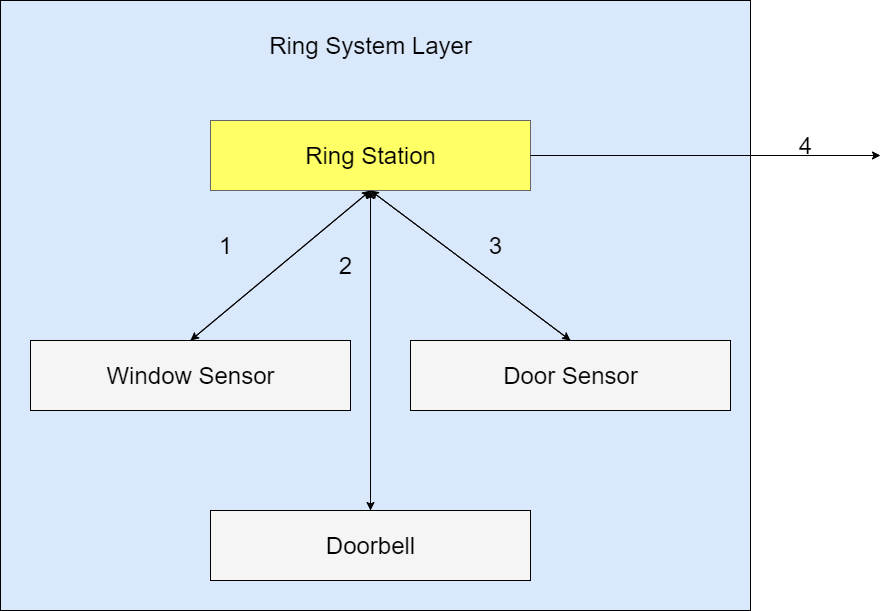
\includegraphics[width=0.60\textwidth]{images/RingLayer.drawio1.png}
 \caption{Ring Base Ring Station Subsystem diagram}
\end{figure}

\subsubsection{Assumptions}
Signals may be intercepted, or flags may be read from the ring doorbell system. We hope to use Ring to help receive signals either away from or outside of the house.

\subsubsection{Responsibilities}
The ring system must be responsible for picking up signals to alert the phone so that the wristband may vibrate.

\subsubsection{Subsystem Interfaces}

\begin {table}[H]
\caption {Ring Station interfaces} 
\begin{center}
    \begin{tabular}{ | p{1cm} | p{6cm} | p{3cm} | p{3cm} |}
    \hline
    ID & Description & Inputs & Outputs \\ \hline
    4 & Ring Station & signals from ring subsystems & notifications  \\ \hline
    \end{tabular}
\end{center}
\end{table}
\newpage

\subsection{Window Sensor}
%This section should be a general description of a particular subsystem for the given layer. For most subsystems, an extract of the architectural block diagram with data flows is useful. This should consist of the subsystem being described and those subsystems with which it communicates.

\begin{figure}[h!]
	\centering
 	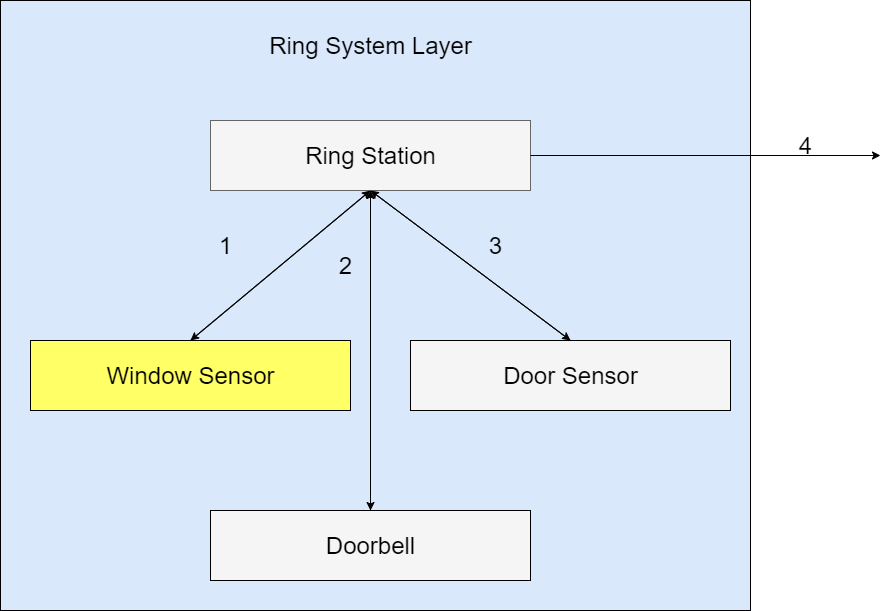
\includegraphics[width=0.60\textwidth]{images/RingLayer.drawio2.png}
 \caption{Ring Base Ring Station Subsystem diagram}
\end{figure}

\subsubsection{Assumptions}
Signals may be intercepted, or flags may be read from the ring doorbell system. We hope to use Ring to help receive signals either away from or outside of the house.

\subsubsection{Responsibilities}
The window sensor will detect if windows in the house are being opened. It will alert the Ring station of this detection.

\subsubsection{Subsystem Interfaces}

\begin {table}[H]
\caption {Window Sensor interfaces} 
\begin{center}
    \begin{tabular}{ | p{1cm} | p{6cm} | p{3cm} | p{3cm} |}
    \hline
    ID & Description & Inputs & Outputs \\ \hline
    2 & Window Sensor & Window Signal Received & Window Flag passed  \\ \hline

    \end{tabular}
\end{center}
\end{table}

\subsection{Doorbell}
%This section should be a general description of a particular subsystem for the given layer. For most subsystems, an extract of the architectural block diagram with data flows is useful. This should consist of the subsystem being described and those subsystems with which it communicates.

\begin{figure}[h!]
	\centering
 	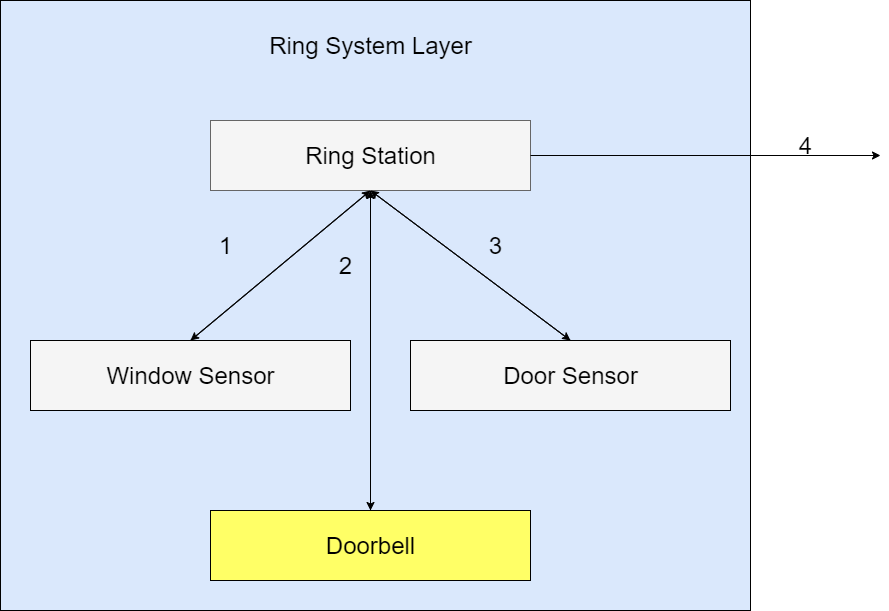
\includegraphics[width=0.60\textwidth]{images/RingLayer.drawio3.png}
 \caption{Ring Base Ring Station Subsystem diagram}
\end{figure}

\subsubsection{Assumptions}
Signals may be intercepted, or flags may be read from the ring doorbell system. We hope to use Ring to help receive signals either away from or outside of the house.

\subsubsection{Responsibilities}
The doorbell will detect the user of people at the door. It will alert the Ring station of this detection.

\subsubsection{Subsystem Interfaces}

\begin {table}[H]
\caption {Doorbell interfaces} 
\begin{center}
    \begin{tabular}{ | p{1cm} | p{6cm} | p{3cm} | p{3cm} |}
    \hline
    ID & Description & Inputs & Outputs \\ \hline
    1 & Doorbell & Ring Doorbell Signal received & Doorbell Flag passed  \\ \hline
    \end{tabular}
\end{center}
\end{table}

\subsection{Door Sensor}
%This section should be a general description of a particular subsystem for the given layer. For most subsystems, an extract of the architectural block diagram with data flows is useful. This should consist of the subsystem being described and those subsystems with which it communicates.

\begin{figure}[h!]
	\centering
 	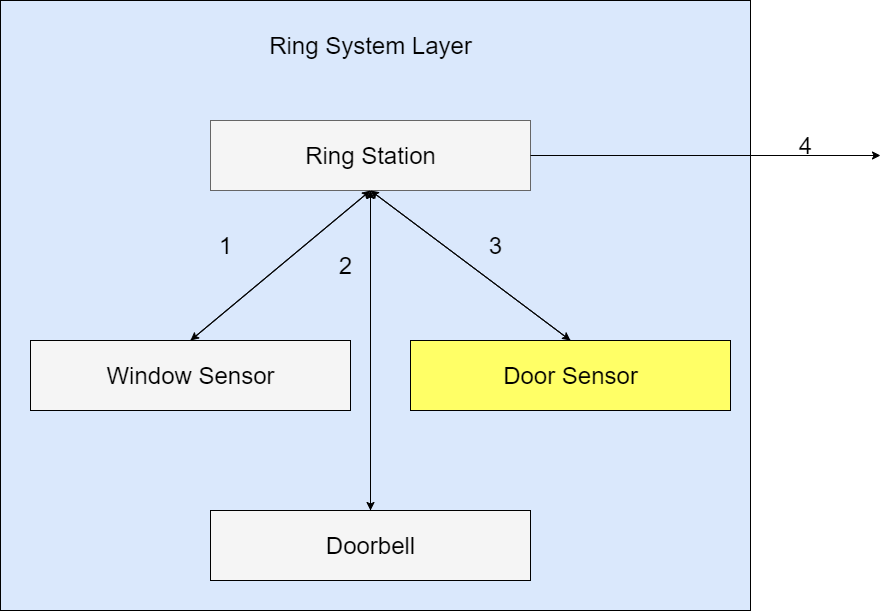
\includegraphics[width=0.60\textwidth]{images/RingLayer.drawio4.png}
 \caption{Ring Base Ring Station Subsystem diagram}
\end{figure}

\subsubsection{Assumptions}
Signals may be intercepted, or flags may be read from the ring doorbell system. We hope to use Ring to help receive signals either away from or outside of the house.

\subsubsection{Responsibilities}
The door sensor will detect if the door is being opened. It will alert the Ring station of this detection.

\subsubsection{Subsystem Interfaces}

\begin {table}[H]
\caption {Ring Station interfaces} 
\begin{center}
    \begin{tabular}{ | p{1cm} | p{6cm} | p{3cm} | p{3cm} |}
    \hline
    ID & Description & Inputs & Outputs \\ \hline
    3 & Door Sensor & Door Signal Received & Door Flag passed  \\ \hline
    \end{tabular}
\end{center}
\end{table}
